
\chapter{Introduction}

\section{Motivation and Objectives}

It has been established via airborne magnetic surveys in the U.S.A. \citep{Donovan} that magnetic contrasts---that is, ``magnetisation that is different from background magnetisation and which may give rise to mappable magnetic anomalies detectable by conventional magnetometry" \citep{Machel}---are a common feature of hydrocarbon reservoir sites. \citet{Donovan} suggested that these magnetic anomalies are caused by near-surface magnetic minerals (specifically, magnetite) induced by upward hydrocarbon seepage from the underlying hydrocarbon reservoir. Further studies by \citet{Donovan2}, \citet{Reynolds} and \citet{Elmore} in the U.S.A., \citet{Diaz}, \citet{Costanzo}, \citet{Guzman}, \citet{Gonzalez} in Venezuela and \citet{Liu3}, \citet{Liu2} and \citet{Liu} in China have provided strong evidence for a genetic relationship between the magnetic contrasts produced by ferrimagnetic minerals near the surface and the underlying reservoir. These investigations confirm the original hypothesis of \citet{Donovan} that the reducing environment caused by the upward seepage from the reservoirs is conducive to the formation of magnetic minerals---such as magnetite and other Fe-oxides, and greigite and other Fe-sulfides---and/or the destruction of minerals such as hematite \citep{Machel} and thus further the case for using a combination of aeromagnetic surveying and rock-magnetic measurements of soils and rocks for cheap hydrocarbon prospecting as proposed by \citet{Donovan2}.\par

Though the discussion on the exact mechanism for the formation of these minerals is ongoing, \citet{Machel} have identified two primary agents for the precipitation of magnetic minerals under the influence of hydrocarbon seepage. At higher temperatures and thus higher depths they propose chemical processes as the main factor while at shallower depths and lower temperatures it is argued that microbial sulfate-reducing processes are playing the larger role. \citet{Machel} also emphasised the difficulty in linking a magnetic anomaly to a process of hydrocarbon seepage because the precipitation of magnetic minerals can cause positive or negative anomalies---that is, peaks or dips in the geomagnetic field and/or the magnetic susceptibility of the soils. Nevertheless, careful analysis of the local conditions can result in the successful application of rock-magnetic measurements to hydrocarbon exploration (see \citet{Liu} and \citet{Donovan2}). Magnetization of oil bearing rocks can also be used to assess the quality of oil as discussed by \citet{Emmerton}.\par

It was recognized by \citet{Reynolds} that in some cases iron sulfides may be more important to the magnetic contrasts and thus to the identification of prospective oil-producing fields than iron oxides. Particularly, greigite has been identified as an authigenic mineral of the utmost importance in the Simpson oil field in Alaska \citep{Reynolds}. Greigite is an iron sulfide (Fe$_3$S$_4$) that can be thought of as the sulfur equivalent of the iron oxide magnetite (Fe$_3$O$_4$) as they have the same crystal structure only with sulfur replacing oxygen. Like magnetite, it is highly magnetic. Nevertheless, since it is thought to be unstable, its importance as a palaeomagnetic recorder has not been as readily realized as that of magnetite. Also, its magnetic parameters were poorly understood until the work of \citet{Chang} who by synthesising highly pure greigite were able to measure the critical magnetic parameters. \citet{Mxwt1} made use of the new accurate measurements of greigite to simulate greigite grains and the effect of intergrain interactions.\par

\citet{Liu} has proposed that magnetic mineral grains that are linked to hydrocarbon seepage have sizes {\raise.17ex\hbox{$\scriptstyle\sim$}}25nm and thus generally in the single domain (SD) range. In terms of morphology, it has been repeatedly found (see \citet{Aldana} and references therein) that roughly spherical grains of magnetite and/or greigite assemble in raspberry-shaped aggregates (see figure (\ref{Fig1})) called framboids (from the french \textit{framboise} meaning raspberry). It is my interest to model these structures via micromagnetics to investigate their domain structure and behaviour in routine rock-magnetic and palaeomagnetic measurements that could also correlate with the size of the aggregates. It is an open question how the intergrain interactions will affect the otherwise simpler problem of modelling single grains, however \citet{Mxwt2}, \citet{Mxwt1} have made a strong case for the importance of intergrain magnetostatic interactions. Further understanding of framboidal aggregates of greigite or magnetite could aid in developing future oil exploration techniques that are cheaper than more conventional techniques vastly used today.
\begin{figure}[ht]
\centering
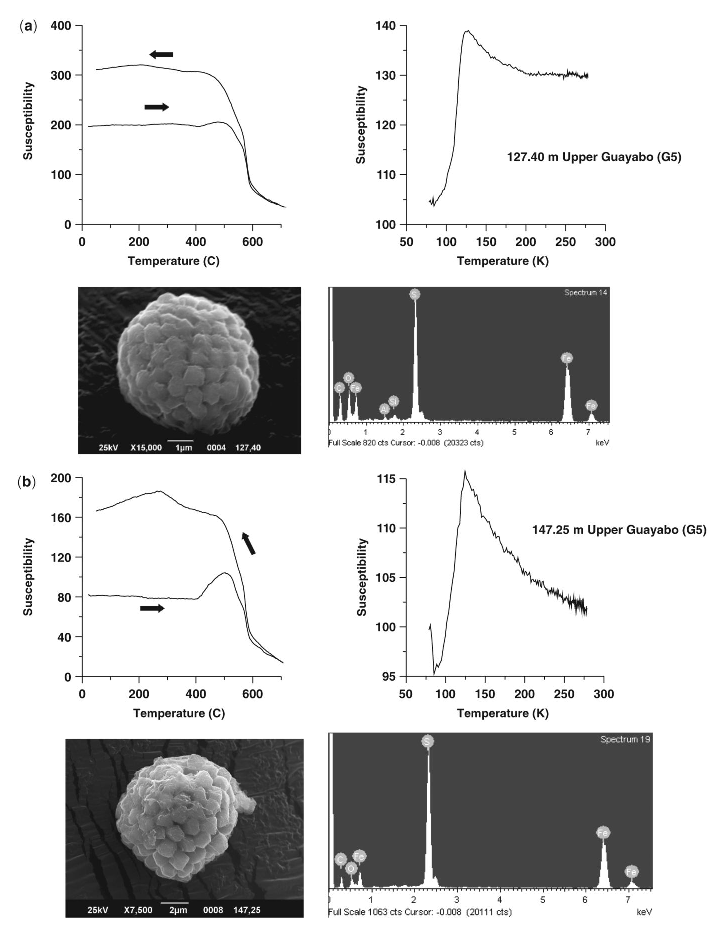
\includegraphics{fram.eps}
\caption{SEM photomicrographs of framboidal Fe- and S-rich magnetic mineral (probably greigite). Taken from \citet{Costanzo2}.}
\label{Fig1}
\end{figure}